%-----------------------------------LICENSE------------------------------------%
%   This file is part of tikz_figures.                                         %
%                                                                              %
%   tikz_figures is free software: you can redistribute it and/or              %
%   modify it it under the terms of the GNU General Public License as          %
%   published by the Free Software Foundation, either version 3 of the         %
%   License, or (at your option) any later version.                            %
%                                                                              %
%   tikz_figures is distributed in the hope that it will be useful,            %
%   but WITHOUT ANY WARRANTY; without even the implied warranty of             %
%   MERCHANTABILITY or FITNESS FOR A PARTICULAR PURPOSE.  See the              %
%   GNU General Public License for more details.                               %
%                                                                              %
%   You should have received a copy of the GNU General Public License along    %
%   with tikz_figures.  If not, see <https://www.gnu.org/licenses/>.           %
%------------------------------------------------------------------------------%

% Use the standalone class for displaying the tikz image on a small PDF.
\documentclass[crop, tikz]{standalone}

% Import the tikz package to use for the drawing.
\usepackage{tikz}

% Needed for blackboard bold C.
\usepackage{amssymb}

% The arrow and decorations packages are used for the LaTeX arrow.
\usetikzlibrary{arrows.meta, decorations.markings}

% Begin the document.
\begin{document}

    % Draw the figure.
    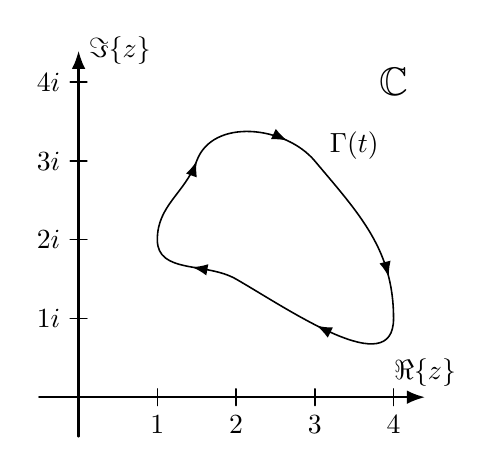
\begin{tikzpicture}[%
        > = Latex,
        line width = 0.2mm,
        line cap = round,
        ->-/.style = {%
            decoration = {%
                markings,
                mark = at position 0.00 with \arrow{>},
                mark = at position 0.15 with \arrow{>},
                mark = at position 0.40 with \arrow{>},
                mark = at position 0.60 with \arrow{>},
                mark = at position 0.80 with \arrow{>}
            },
            postaction = {decorate}
        }
    ]

        % Coordinates for the points in the curve.
        \coordinate (P0) at (1.5, 3.0);
        \coordinate (P1) at (3.0, 3.0);
        \coordinate (P2) at (4.0, 1.0);
        \coordinate (P3) at (2.0, 1.5);
        \coordinate (P4) at (1.0, 2.0);

        % Axes:
        \begin{scope}[thick]
            \draw[->] (-0.5, 0.0) to (4.4, 0.0) node [above] {$\Re\{z\}$};
            \draw[->] (0.0, -0.5) to (0.0, 4.4) node [right] {$\Im\{z\}$};
        \end{scope}

        % Axes labels:
        \foreach\n in {1, 2, 3, 4}{%
            \draw (\n, 3pt) to (\n, -3pt) node [below] {$\n$};
            \draw (3pt, \n) to (-3pt, \n) node [left]  {$\n{i}$};
        }

        % Draw the Jordan Curve.
        \draw[->-]
            (P0) to [out = 70, in = 130]
            (P1) to [out = -50, in = 90]
            (P2) to [out = -90, in = -30]
            (P3) to [out = 150, in = -90]
            (P4) to [out = 90, in = -110] cycle;

        % Labels for the complex plane and the Jordan curve.
        \node at (4.0, 4.0) {\Large{$\mathbb{C}$}};
        \node at (3.5, 3.2) {\normalsize{$\Gamma(t)$}};
    \end{tikzpicture}
\end{document}
